\section{Construction of the model differential equations}
Section \ref{part} showed how the various components of point and
distributed input can be partitioned between the proximal and
distal boundaries of a segment. Once the total axial current
$I_\mathrm{PD}+I_\mathrm{P}$ at the proximal boundary of a segment
and $I_\mathrm{PD}+I_\mathrm{D}$ at the distal boundary of a
segment are determined, the family of ordinary differential
equations modelling the branched dendrite is constructed by
enforcing conservation of current at all segment boundaries.

Each dendritic terminal at which the potential is unknown
contributes one differential equation with form determined by the
properties of the terminal. For example, if the terminal is
sealed, the differential equation expresses the condition
$I_\mathrm{PD}+I_\mathrm{D}=0$. At a dendritic branch point, the
single differential equation is formed by equating the sum of the
proximal current in the child segments to the distal current in
the parent segment. A point soma behaves like a branch point with
the current crossing the somal membrane playing the role of the
distal current in the parent segment. Finally, at all other
segment boundaries, the differential equation is constructed by
equating the distal current of one segment to the proximal current
of its neighbour.

Suppose that there are $m$ nodes at which the potential is
unknown, then the compartmental model of the neuron will be
written for the potentials
\begin{equation}\label{cmde1}
V(t)=\big[\,V_1(t),V_2(t),\cdots,V_m(t)\,]^\mathrm{T}\,.
\end{equation}
where $V_k(t)$ is the potential at the $k^{th}$ node. The system
of differential equations satisfied by $V(t)$ has general form
\begin{equation}\label{gmde2}
C\,\frac{dV}{dt}+G_\mathrm{SYN}(t)\,V+G_\mathrm{IVDC}(\bs{\theta}(t))\,V-AV+I(t)=0
\end{equation}
where $C$, $G_\mathrm{SYN}(t)$, $G_\mathrm{IVDC}(\bs{\theta}(t))$
and $A$ are $m\times m$ matrices such that their $(j,k)^{th}$
entry is non-zero whenever the $j^{th}$ and $k^{th}$ nodes lie at
opposite ends of a segment, \emph{i.e.}, they are neighbouring
nodes. In equation (\ref{gmde2}), $A$ is a constant matrix of
axial conductances and $C$ is a constant matrix of capacitances.
The function $G_\mathrm{SYN}(t)$ is a matrix of time-dependent
conductances associated with synaptic input to the dendrite, the
function $G_\mathrm{IVDC}(\bs{\theta}(t))$ is a matrix of
time-dependent conductances associated with intrinsic
voltage-dependent transmembrane current to the dendrite, and
$I(t)$ is a column vector of voltage-independent currents.
Equation (\ref{gmde2}) is integrated over the interval $[t,t+h]$
to get
\begin{equation}\label{gmde3}
\begin{array}{l}
\ds C\big[\,V(t+h)-V(t)\big]+\int_t^{t+h}
G_\mathrm{SYN}(t)V(t)\,dt+\int_t^{t+h}
G_\mathrm{IVDC}(\bs{\theta}(t))V(t)\,dt\\[10pt]
\qquad\qquad\ds-\;A\int_t^{t+h} V(t)\,dt+\int_t^{t+h} I(t)\,dt=0
\,.
\end{array}
\end{equation}
The trapezoidal rule is used to estimate each integral in equation
(\ref{gmde3}) with the exception of the integral of intrinsic
voltage-dependent current which is estimated by the midpoint rule.
The result of this calculation is
\begin{equation}\label{gmde4}
\begin{array}{l}
\ds C \big[V(t+h)-V(t)\big]+\frac{h}{2}
\Big[G_\mathrm{SYN}(t+h)V(t+h)+G_\mathrm{SYN}(t)V(t)\Big]\\[10pt]
\ds\qquad+\;h G_\mathrm{IVDC}\big(\bs{\theta}(t+h/2)\big) V(t+h/2)
-\frac{h}{2} \Big[A V(t+h)+AV(t)\Big]\\[10pt]
\ds\qquad\qquad\ds+\;\frac{h}{2}\Big[I(t+h)+I(t)\Big] +O(h^3)=0\,.
\end{array}
\end{equation}
By noting that $2V(t+h/2)=V(t+h)+V(t)+O(h^2)$, equation
(\ref{gmde4}) may be rearranged to give
\begin{equation}\label{mde6}
\begin{array}{l}
\ds \Big[2C-hA+h\,G_\mathrm{SYN}(t+h)
+h\,G_\mathrm{IVDC}\big(\bs{\theta}(t+h/2)\big)\,\Big]\,V(t+h) =
\\[10pt] \quad\ds \Big[\,2C+h\,A-h\,G_\mathrm{SYN}(t)
-h\,DG_\mathrm{IVDC}\big(\bs{\theta}(t+h/2)\big)\,\Big]\,V(t)
-h\Big[I(t+h)+I(t)\Big]+O(h^3).
\end{array}
\end{equation}
The computation of $G_\mathrm{IVDC}\big(\bs{\theta}(t+h/2)\big)$
depends on how intrinsic voltage-dependent current is specified.
For example, for a membrane following Hodgkin-Huxley kinetics,
$G_\mathrm{IVDC}\big(\bs{\theta}(t+h/2)\big)$ is specified in
terms of the solutions of a set of auxiliary equations. In this
case, it is well known that
$G_\mathrm{IVDC}\big(\bs{\theta}(t+h/2)\big)$ can be computed to
adequate accuracy from $V(t)$ and the differential equations
satisfied by the auxiliary variables (\emph{e.g.}, see Lindsay
\emph{et al.}, \cite{Lindsay01a}). The coefficient matrices in
equation (\ref{mde6}) are therefore determined by $V(t)$ and known
prior to the determination of the potential $V(t+h)$.

\subsection{Some additional comments}
All compartmental models of a dendrite begin with a subdivision of
its sections into contiguous segments. The segments, in turn,
define the compartments of the mathematical model. Both the new
and traditional compartmental models are based on the \emph{same}
morphological segments. In a traditional compartmental model, the
distribution of membrane potential throughout a dendrite is
described by the membrane potentials at the centres of dendritic
segments. By contrast, in the new compartmental model the membrane
potential throughout a dendrite is described by the potential at
segment endpoints. The number of nodes at which potentials are to
be determined, and consequently the numerical complexity of the
problem, are identical in both types of compartmental model.
Furthermore, both models involve nearest neighbour interactions,
and so the structure of the differential equations describing
either model is identical. Consequently benefits such as the
existence of a sparse matrix factorisation of the matrix on the
left hand side of equation (\ref{mde6}) are enjoyed by both types
of model.

Finally, it should be noted that the development of the new
compartmental model highlights structural differences between the
treatment of point input in this model and their treatment in a
numerical procedure used to solve the partial differential
equations of the continuum model. In the compartmental model,
conservation of current is applied at each synapse to arrive at an
equation connecting potentials at neighbouring nodes. In a
numerical procedure (\emph{e.g.}, finite elements or finite
differences), the potential at synapses is estimated on the basis
of the assumed representation of the potential between nodes.
Consequently, numerical procedures often conserve current in an
averaged sense, but not necessarily point-wise at a synapse. It is
unclear to what extent such a treatment of synaptic input
influences the accuracy of numerical schemes.

\section{The model neuron}
The comparison of the accuracy of the traditional and new
compartmental models is based on the construction of a branched
neuron for which the continuum model has a closed form expression
for the membrane potential in response to exogenous input. This
solution then stands as a reference against which the performance
of the traditional and new compartmental models can be assessed.
The most effective way to construct a branched model neuron with a
closed form solution for the membrane potential is to choose the
radii and lengths of its sections such that the Rall conditions
for an equivalent cylinder are satisfied (Rall, \cite{Rall64}).
These conditions require that the sum of the three-halves power of
the diameters of the child limbs is equal to the three-halves
power of the diameter of the parent limb at any branch point, and
that the total electrotonic length from a branch point to
dendritic tip is independent of path. In particular, the
electrotonic distance from soma-to-tip is independent of path. The
model neuron used in our simulation exercises, illustrated in
Figure \ref{TestNeuron}, satisfies these conditions. When the Rall
conditions are satisfied, the effect at the soma of any
configuration of input on the branched model of the neuron is
identical to the effect at the soma of the unbranched equivalent
cylinder with biophysical properties and configuration of input
determined uniquely from those of the original branched neuron
(Lindsay \emph{et al.}, \cite{Lindsay03}).

\begin{figure}[!h]
\[
\begin{array}{c}
$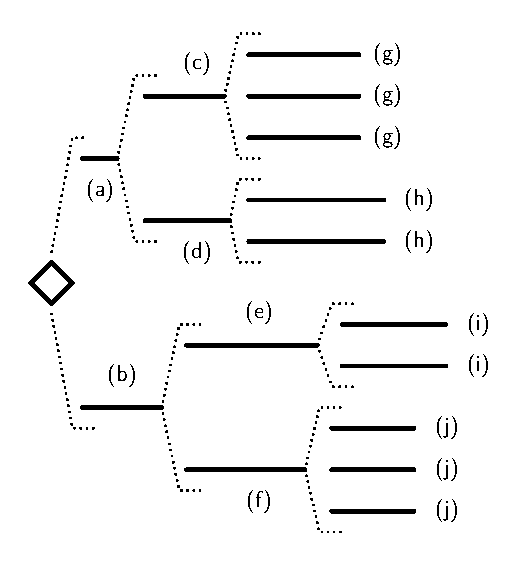
\includegraphics[ ]{NewCompFig4.eps}$
\end{array}\qquad
\begin{array}{ccc}
\hline
\mbox{Section} & \mbox{Length }\mu\mbox{m} & \mbox{Diameter }\mu\mbox{m}\\[2pt]
\hline
 (a) & 166.809245 & 7.089751 \\
 (b) & 379.828386 & 9.189790 \\
 (c) & 383.337494 & 4.160168 \\
 (d) & 410.137845 & 4.762203 \\
 (e) & 631.448520 & 6.345604 \\
 (f) & 571.445800 & 5.200210 \\
 (g) & 531.582750 & 2.000000 \\
 (h) & 651.053246 & 3.000000 \\
 (i) & 501.181023 & 4.000000 \\
 (j) & 396.218388 & 2.500000 \\
\hline
\end{array}
\]
\centering
\parbox{5.5in}{\caption{\label{TestNeuron} A branched neuron
satisfying the Rall conditions. The diameters and lengths of the
dendritic sections are given in the right hand panel of the
figure. At each branch point, the ratio of the length of a section
to the square root of its radius is fixed for all children of the
branch point.}}
\end{figure}

%\begin{figure}[!h]
%\[
%\begin{array}{c}
%$\begin{mfpic}[1][1]{0}{220}{-20}{220}
%\pen{2pt}
%\dotsize=1pt
%\dotspace=3pt
%\lines{(-5,100),(5,110),(15,100),(5,90),(-5 ,100)}
%% Upper dendrite
%% Root branch
%\dotted\lines{(5,115),(15,170),(20,170)}
%\lines{(20.0,160),(36.7,160)}
%\tlabel[tc](28.4,150){\textsf{(a)}}
%% Level 1
%\lines{(50.0,190),(88.3,190)}
%\tlabel[bc](75,200){\textsf{(c)}}
%\lines{(50.0,130),(91.0,130)}
%\tlabel[tc](75,120){\textsf{(d)}}
%\dotted\lines{(36.7,160),(45,200),(55,200)}
%\dotted\lines{(36.7,160),(45,120),(55,120)}
%% Level 2
%\lines{(100.0,210),(153.2,210)}
%\lines{(100.0,190),(153.2,190)}
%\lines{(100.0,170),(153.2,170)}
%\tlabel[cl](160,210){\textsf{(g)}}
%\tlabel[cl](160,190){\textsf{(g)}}
%\tlabel[cl](160,170){\textsf{(g)}}
%\dotted\lines{(88.3,190),(95,220),(105,220)}
%\dotted\lines{(88.3,190),(95,160),(105,160)}
%\lines{(100.0,140),(165.1,140)}
%\lines{(100.0,120),(165.1,120)}
%\dotted\lines{(91.0,130),(95,150),(105,150)}
%\dotted\lines{(91.0,130),(95,110),(105,110)}
%\tlabel[cl](175,140){\textsf{(h)}}
%\tlabel[cl](175,120){\textsf{(h)}}
%%
%% Lower dendrite
%% Root branch
%\lines{(20.0,40),(58.0,40)}
%\dotted\lines{(5,85),(15,30),(25,30)}
%\tlabel[bc](39,50){\textsf{(b)}}
%% Level 1
%\lines{(70.0,70),(133.1,70)}
%\lines{(70.0,10),(127.1,10)}
%\dotted\lines{(58,40),(66.5,80),(76.5,80)}
%\dotted\lines{(58,40),(66.5,0),(76.5,0)}
%\tlabel[bc](105,80){\textsf{(e)}}
%\tlabel[tc](105,0){\textsf{(f)}}
%% Level 2
%\lines{(145,80),(195.1,80)}
%\lines{(145,60),(195.1,60)}
%\dotted\lines{(133.1,70),(140,90),(150,90)}
%\dotted\lines{(133.1,70),(140,50),(150,50)}
%\tlabel[cl](205,80){\textsf{(i)}}
%\tlabel[cl](205,60){\textsf{(i)}}
%\lines{(140,30),(179.6,30)}
%\lines{(140,10),(179.6,10)}
%\lines{(140,-10),(179.6,-10)}
%\dotted\lines{(127.1,10),(134,40),(144,40)}
%\dotted\lines{(127.1,10),(134,-20),(144,-20)}
%\tlabel[cl](190,30){\textsf{(j)}}
%\tlabel[cl](190,10){\textsf{(j)}}
%\tlabel[cl](190,-10){\textsf{(j)}}
%\end{mfpic}$
%\end{array}\qquad
%\begin{array}{ccc}
%\hline
%\mbox{Section} & \mbox{Length }\mu\mbox{m} & \mbox{Diameter }\mu\mbox{m}\\[2pt]
%\hline
% (a) & 166.809245 & 7.089751 \\
% (b) & 379.828386 & 9.189790 \\
% (c) & 383.337494 & 4.160168 \\
% (d) & 410.137845 & 4.762203 \\
% (e) & 631.448520 & 6.345604 \\
% (f) & 571.445800 & 5.200210 \\
% (g) & 531.582750 & 2.000000 \\
% (h) & 651.053246 & 3.000000 \\
% (i) & 501.181023 & 4.000000 \\
% (j) & 396.218388 & 2.500000 \\
%\hline
%\end{array}
%\]
%\centering
%\parbox{5.5in}{\caption{\label{TestNeuron} A branched neuron
%satisfying the Rall conditions. The diameters and lengths of the
%dendritic sections are given in the right hand panel of the
%figure. At each branch point, the ratio of the length of a section
%to the square root of its radius is fixed for all children of the
%branch point.}}
%\end{figure}

To guarantee that any apparent errors between the closed form
solution and the numerical solution from either compartmental
model are not due to the lack of precision with which the branched
dendrite is represented as an equivalent cylinder, a high degree
of accuracy is used in the specification of dendritic radii and
section lengths in the model neuron. The model neuron illustrated
in Figure \ref{TestNeuron} is assigned a specific membrane
conductance of $0.091\,$mS/cm$^2$ ($g_\mathrm{M}$) and specific
membrane capacitance of $1.0\,\mu$F/cm$^2$ ($c_\mathrm{M}$), and
axoplasm of conductance $14.286\,$mS/cm ($g_\mathrm{A}$). With
these biophysical properties, the equivalent cylinder has length
one electrotonic unit. The soma of the test dendrite is assumed to
have membrane area $A_\mathrm{S}$, specific conductance
$g_\mathrm{S}=g_\mathrm{M}$ and specific capacitance
$c_\mathrm{S}=c_\mathrm{M}$.

\subsection{Analytical solution}
It may be shown that $V(t)$, the deviation of the somal
transmembrane potential from its resting value as a result of a
distribution $\mathcal{I}(x,t)$ of current on a uniform
cylindrical dendrite of radius $a$ and length $l$ attached to a
soma is
\begin{equation}\label{es4}
V(t)=e^{-t/\tau}\,\Big[\,\phi_0(t)+\sum_\beta\;\phi_\beta(t)
e^{-\beta^2 t/L^2\tau}\,\cos\beta\,\Big]\,, \qquad
L=l\,\sqrt{\ds\frac{2 g_\mathrm{M}}{a g_\mathrm{A}}}
\end{equation}
where $\tau$ is the time constant of the somal and dendritic
membranes and $g_\mathrm{M}$ and $g_\mathrm{A}$ have their usual
meanings. The summation is taken over all the solutions $\beta$ of
the transcendental equation $\tan\beta+\gamma\beta=0$ where
$\gamma$ (constant) is the ratio of the total membrane area of the
soma to the total membrane area of the dendrite. The functions
$\phi_0(t)$ and $\phi_\beta(t)$ are solutions of the differential
equations
\begin{equation}\label{es9}
\begin{array}{rcl}
\ds\frac{d\phi_0}{dt} & = & -\ds\frac{e^{t/\tau}}
{C_\mathrm{D}+C_\mathrm{S}}\,\Big[\,
\mathcal{I}_\mathrm{S}(t)+\int_0^l\,\mathcal{I}(x,t)\,dx\,\Big]\,,\\[10pt]
\ds\frac{d\phi_\beta}{dt} & = &
-\ds\frac{2e^{(1+\beta^2/L^2)t/\tau}} {C_\mathrm{D}
+C_\mathrm{S}\cos^2\beta}\,\Big[\,
\int_0^1\,\mathcal{I}(x,t)\cos\beta\big(1-x/l\big)\,dx
+\cos\beta\,\mathcal{I}_\mathrm{S}(t)\,\Big]
\end{array}
\end{equation}
with initial conditions $\phi_0(0)=\phi_\beta(0)=0$, that is, the
neuron is initialised at its resting potential. The parameters
$C_\mathrm{S}$ and $C_\mathrm{D}$ denote respectively the total
membrane capacitances of the soma and dendrite, and
$\mathcal{I}_\mathrm{S}(t)$ is the current supplied to the soma.

In the special case in which point currents $\mathcal{I}_1(t),
\cdots,\mathcal{I}_n(t)$ act at distances $x_1,\cdots x_n$ from
the soma of the uniform cylinder, the corresponding coefficient
functions $\phi_0$ and $\phi_\beta$ satisfy
\begin{equation}\label{ec2}
\begin{array}{rcl}
\ds\frac{d\phi_0}{dt} & = &\ds -\frac{e^{t/\tau}}
{C_\mathrm{D}+C_\mathrm{S}}\,\Big[\,
\mathcal{I}_\mathrm{S}(t)+\sum_{k=1}^n\;\mathcal{I}_k(t)\,\Big]\,,\\[10pt]
\ds\frac{d\phi_\beta}{dt} & = &
\ds-\frac{2e^{(1+\beta^2/L^2)t/\tau}}
{C_\mathrm{D}+C_\mathrm{S}\cos^2\beta}\,\Big[\, \sum_{k=1}^n
\;\mathcal{I}_k(t)\cos\beta\big(1-x_k/l\big)
+\cos\beta\,\mathcal{I}_\mathrm{S}(t)\,\Big]\,.
\end{array}
\end{equation}
